\documentclass[12pt]{beamer}
\usetheme{COURS}
\usepackage{tcolorbox}
\usepackage{textpos}


\def\red{\color{red}}
\def\blue{\color{blue}}
\def\green{\color{green}}

\def\opstyle#1{\ensuremath{\operatorname{#1}}}


\title[Algorithmes combinatoires]%
{\bf Comptage et énumération de structures de données:
  \\ Algorithmes efficaces et implantations optimisées
}
\author{\textbf{\Large Florent Hivert}\\[5mm]
  Mél : \texttt{Florent.Hivert@lri.fr}\\
  Adresse universelle : \texttt{http://www.lri.fr/\~{ }hivert}
}
\date{}

\begin{document}
\newcommand{\Count}{\opstyle{count}}
\newcommand{\List}{\opstyle{list}}
\newcommand{\Iter}{\opstyle{iter}}
\newcommand{\Unrank}{\opstyle{unrank}}
\newcommand{\Rank}{\opstyle{rank}}
\newcommand{\First}{\opstyle{first}}
\newcommand{\Next}{\opstyle{next}}
\newcommand{\Random}{\opstyle{random}}
\newcommand{\Oh}{O}

%***********************************************************************
\frame{\titlepage}

%\begin{frame}
%   \slidepagestyle{empty}
%   \addtocounter{frame}{-1}
%   \maketitle
%\end{frame}

%***********************************************************************

\begin{frame}{Manipulation d'ensembles finis:}
  ... mais souvent très grand ...
  \begin{itemize}
  \item suites de 64~bits: \texttt{0xce24762189cdef0d}
  \item permutés d'un tableaux: \texttt{[5,3,6,4,1,2]}
  \item arbres binaires à $7$~noeuds: \raisebox{-1cm}{\tiny\newcommand{\nodea}{\node[draw,circle] (a) {$$};}
 \newcommand{\nodeb}{\node[draw,circle] (b) {$$};}
 \newcommand{\nodec}{\node[draw,circle] (c) {$$};}
 \newcommand{\noded}{\node[draw,circle] (d) {$$};}
 \newcommand{\nodee}{\node[draw,circle] (e) {$$};}
 \newcommand{\nodef}{\node[draw,circle] (f) {$$};}
 \newcommand{\nodeg}{\node[draw,circle] (g) {$$};}\begin{tikzpicture}[auto]
\matrix[anchor=west,column sep=.05cm, row sep=.1cm,ampersand replacement=\&]{
         \&         \&         \&         \&         \& \nodea  \&         \&         \&         \\ 
         \&         \&         \& \nodeb  \&         \&         \&         \& \nodef  \&         \\ 
         \& \nodec  \&         \&         \&         \&         \& \nodeg  \&         \&         \\ 
 \noded  \&         \& \nodee  \&         \&         \&         \&         \&         \&         \\
};
\path[ultra thick, red] (c) edge (d) edge (e)
	(b) edge (c)
	(f) edge (g)
	(a) edge (b) edge (f);
\end{tikzpicture}}
  \item graphes à $8$-sommets:
    \raisebox{-1cm}{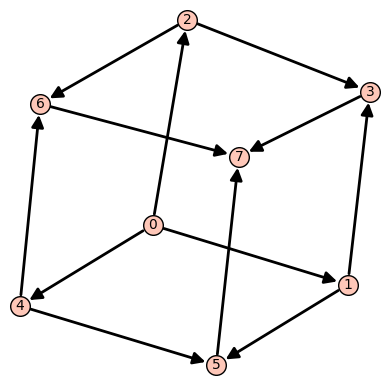
\includegraphics[width=2cm]{media/graphe.png}}
  \item document XML à $n$ balises
  \item programmes à $n$ caractères en C, chemin d'execution
  \end{itemize}
\end{frame}

\begin{frame}{Objectifs:}

  \begin{tcolorbox}
    \textbf{Algorithmes et implantations efficaces} pour
    \begin{itemize}
    \item Compter, trouver la liste, itérer
    \medskip
    \item recherche d'un élément
    \medskip
    \item Tirage aléatoire équitable
    \end{itemize}
  \end{tcolorbox}
  \bigskip\pause

  Plan:
  \begin{itemize}
  \item Problèmes d'énumeration, objets combinatoires de base
    \medskip

  \item Backtracking, algorithmes lexicographiques, code Gray
    \medskip

  \item Optimisation et parallélisation d'une recherche
  \end{itemize}
\end{frame}


\begin{frame}{Applications}

  \begin{itemize}
  \item \textbf{recherche de solution} par la force brute
    \bigskip

  \item analyse d'algorithmes, \textbf{calcul de complexité}
    \bigskip

  \item \textbf{tests} de programmes, de systèmes
    \bigskip

  \item \textbf{recherche} de failles, fuzzing
    \bigskip

  \item bio-informatique, chimie, physique statistique
  \end{itemize}
\end{frame}

\begin{frame}{Références}

  \begin{itemize}
  \item Frank Ruskey, \textit{Combinatorial Generation}
    \url{doi:10.1.1.93.5967}, 2003, non publié
    \bigskip

  \item A.~Nijenhuis and H.S.~Wilf, \textit{Combinatorial algorithms}, 2nd
    ed., Academic Press, 1978\\
    \url{http://www.math.upenn.edu/~wilf/website/CombinatorialAlgorithms.pdf}
    \bigskip

  \item The (Combinatorial) Object Server : \url{http://sue.csc.uvic.ca/~cos/}
    \bigskip

  \item The On-Line Encyclopedia of Integer Sequences \url{http://oeis.org}
  \end{itemize}
  \begin{textblock*}{100mm}(.75\textwidth,-8.2cm)
    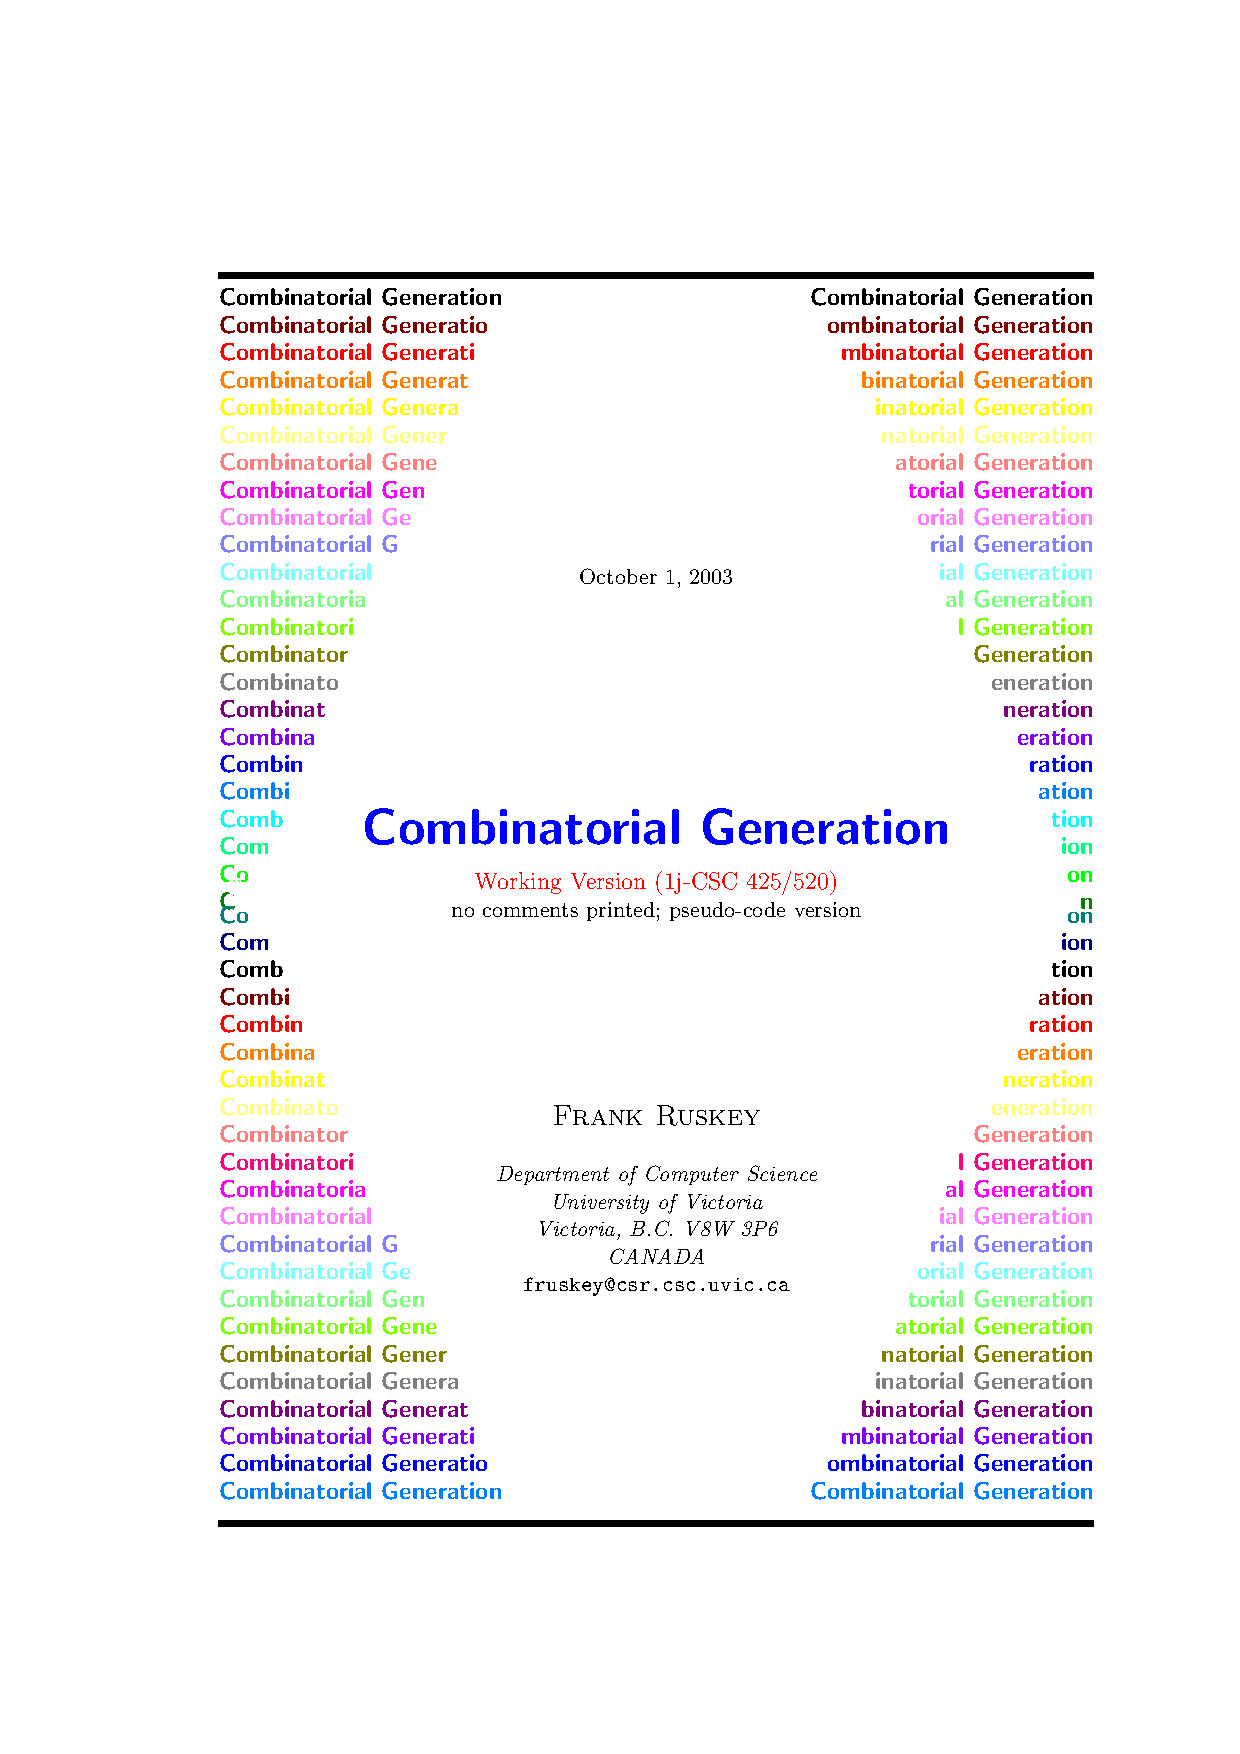
\includegraphics[width=2cm]{media/RuskeyCombGen-1.pdf}
  \end{textblock*}
\end{frame}


\end{document}
